\newcommand{\defs}{../defs}
\documentclass[12pt,oneside,chapterprefix=true]{scrbook}

\usepackage[T1]{fontenc}
\usepackage[utf8x]{inputenc}
\usepackage[brazilian]{babel}
\usepackage[table]{xcolor}
\usepackage{minted}
\usepackage[a5paper,left=0.7cm,right=0.7cm,top=2cm,bottom=2.5cm,]{geometry}
\usepackage{url}
\usepackage{graphicx}
\usepackage[export]{adjustbox}
\usepackage{hyperref}
\usepackage[square]{natbib}
\usepackage[parfill]{parskip}
\usepackage{mdframed}
\usepackage{longtable}
\usepackage{soul}
\usepackage{tabularx}
\usepackage[shortlabels]{enumitem}
\usepackage{xifthen}
\usepackage{multirow}
\usepackage[portuguese, ruled, vlined, linesnumbered, algochapter]{algorithm2e}
\usepackage{amsmath}
\usepackage{amssymb}
\usepackage{amsthm}
\usepackage{tablefootnote}
\usepackage{subfigure}
\usepackage{gensymb}
\usepackage{pgfplots}
\usepackage{xpatch}
\usepackage{varwidth}
\usepackage[htt]{hyphenat}

\renewcommand{\familydefault}{\sfdefault}

\newcommand{\name}{Prof. Marcelo de Souza}
\newcommand{\email}{marcelo.desouza@udesc.br}
\newcommand{\course}{Bacharelado em Engenharia de Software}
\newcommand{\university}{Universidade do Estado de Santa Catarina}
\newcommand{\campus}{Centro de Educação Superior do Alto Vale do Itajaí}
\newcommand{\shortuniversity}{UDESC Ibirama}
\newcommand{\version}{Versão compilada em \today}
\newcommand{\exercisedescription}{Exercício}

\usepackage[automark,headsepline,footsepline]{scrlayer-scrpage}
\lehead{\content}
\lohead{\content}
\rehead{}
\rohead{}
\cehead{}
\cohead{}
\lefoot{\name}
\lofoot{\name}
\refoot{\\\thepage}
\rofoot{\\\thepage}
\cofoot{}
\cefoot{}
\setkomafont{pagehead}{\normalfont\small}
\setkomafont{pagefoot}{\normalfont}

\newpairofpagestyles{firstpage}{}

\newcommand{\makeheader}{
	\thispagestyle{firstpage}
	\vspace*{-42pt}
	\framebox[\textwidth]{
		\parbox{0.97\textwidth}{
			\begin{center}
				{\scriptsize\shortcourse\ -- \class}
				
				\vspace{10pt}
				
				\textbf{\content}
				
				\vspace{2pt}
				
				{\small\name}
				
				\vspace{10pt}
				
				{\scriptsize\shortuniversity\hfill\email}
				
				\vspace{-5pt}
				
				{\scriptsize\course\hfill\version}
				
			\end{center}
		}
	}
%	\vspace{-15pt}
%	\begin{flushright}
%		{\scriptsize\source}
%	\end{flushright}
	\smallskip
}

\renewcommand{\thesection}{\arabic{section}}

\allowdisplaybreaks

\hypersetup{
	colorlinks,
	linkcolor={blue!80!black},
	citecolor={blue!80!black},
	urlcolor={blue!80!black}
}

\definecolor{codelinecolor}{gray}{.90}
\colorlet{codeboxcolor}{blue!8}

\surroundwithmdframed{minted}

\BeforeBeginEnvironment{mdframed}{}
\AfterEndEnvironment{mdframed}{}

\mdfsetup{%
	backgroundcolor=codeboxcolor,
	linecolor=white}

\setminted{%
	mathescape,
	escapeinside=@@,
	linenos,
	breaklines,
	tabsize=3,
	fontsize=\footnotesize}

\newcommand{\code}[1]{%
	\sethlcolor{codelinecolor}
	\texttt{\hl{#1}}%
}

\newcommand{\inblock}[1]{%
	\sethlcolor{blockcolor}
	\hl{\mbox{#1}}%
}

\newcommand{\javacode}[1]{%
	\mintinline[escapeinside=~~]{java}{#1}
}

\newcommand{\javacodecolor}[1]{%
	\mintinline[escapeinside=~~,bgcolor=codeboxcolor]{java}{#1}
}

\newcounter{number}
\newenvironment{exercise}[1][]
{%
	\refstepcounter{number}%
	\noindent%
	\ifthenelse{\equal{#1}{}}%
		{\textbf{\exercisedescription~\thenumber.\\}}%
		{\textbf{\exercisedescription~\thenumber. (#1)\\}}%
	\rmfamily%
}{\medskip}%

\newcommand{\resetexercisenumbering}{
	\setcounter{number}{0}
}

\newcounter{solutionnumber}
\newenvironment{solution}[1][]
{%
	\refstepcounter{solutionnumber}%
	\noindent%
	\ifthenelse{\equal{#1}{}}%
	{\textbf{Solução -- \exercisedescription~\thesolutionnumber.\\}}%
	{\textbf{Solução -- \exercisedescription~\thesolutionnumber. (#1)\\}}%
	\rmfamily%
}{\medskip}%

\makeatletter%
\setlength{\@fptop}{5pt}

\def\arraystretch{1.5}

\newcommand{\insertspace}{\vspace{1.2em}}
\newcommand{\removespace}{\vspace{-1.2em}}

\setlength{\fboxsep}{0.8em}

\usepackage{array}
\newcolumntype{L}[1]{>{\raggedright\let\newline\\\arraybackslash\hspace{0pt}}m{#1}}
\newcolumntype{C}[1]{>{\centering\let\newline\\\arraybackslash\hspace{0pt}}m{#1}}
\newcolumntype{R}[1]{>{\raggedleft\let\newline\\\arraybackslash\hspace{0pt}}m{#1}}

\colorlet{blockcolor}{red!25}
\colorlet{redtext}{red!60!black}

\newcommand{\block}[1]{%
	\medskip
	\begin{figure}[H]
		\centering
		\begin{tikzpicture}
		\node [rectangle, align=center, fill=blockcolor, rounded corners=0.04cm, opacity = 1, text opacity = 1] {%
			#1
		};
		\end{tikzpicture}
	\end{figure}
}

\newcommand{\newtitle}[1]{%
	\begin{figure}[H]
		\begin{tikzpicture}
		\node [rectangle, fill=blue!30, rounded corners=0.04cm, opacity=1, text opacity=1, minimum width=\textwidth, text width=\linewidth-2*\pgfkeysvalueof{/pgf/inner xsep}, align=left] {%
			\textbf{#1}
		};
		\end{tikzpicture}
	\end{figure}
	\vspace{-10pt}
}

\renewcommand{\qedsymbol}{$\blacksquare$}
\xpatchcmd{\proof}{\itshape}{\normalfont\bfseries}{}{}

\newcommand{\content}{Pilhas, filas e deques}
\newcommand{\class}{Algoritmos e Estruturas de Dados}
\newcommand{\shortcourse}{45EST}

\begin{document}

\makeheader

{
Leitura obrigatória:
\begin{itemize}
	\item Capítulo 6 de~\cite{GoodrichEtAl2014} -- Pilhas, filas e deques.
\end{itemize}

Leitura complementar:
\begin{itemize}
	\item Capítulo 6 de~\cite{Preiss2001} -- Pilhas, filas e deques.
\end{itemize}
}

\medskip

\newtitle{Pilhas}

Ideia geral:
\begin{itemize}
	\item Estratégia \textbf{LIFO}: \textit{last-in-first-out}.
	\item Último elemento a ser inserido é o primeiro a ser removido.
	\item {\color{redtext} Simples, eficiente e muito utilizada.}
	\item Operações:
	\begin{itemize}
		\item \texttt{push}: insere elemento no topo da pilha.
		\item \texttt{pop}: remove elemento do topo da pilha.
	\end{itemize}
	\item Aplicações:
	\begin{itemize}
		\item Histórico de acesso de um navegador.
		\item Operações em um editor de texto (desfazer).
	\end{itemize}
\end{itemize}

\clearpage

\begin{itemize}
	\item Exemplo ilustrativo:
\end{itemize}

\begin{figure}[H]
	\centering
	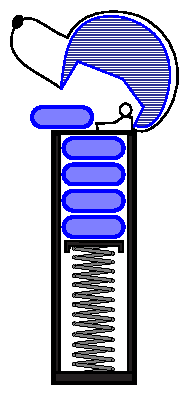
\includegraphics[width=0.21\linewidth]{img/figure-6-1}
\end{figure}

\begin{itemize}
	\item Exemplo de funcionamento:
	\begin{itemize}
		\item Operações de atualização: \texttt{push}, \texttt{pop}.
		\item Operações auxiliares: \texttt{size}, \texttt{top}, \texttt{isEmpty}.
	\end{itemize}
\end{itemize}

\begin{figure}[H]
	\centering
	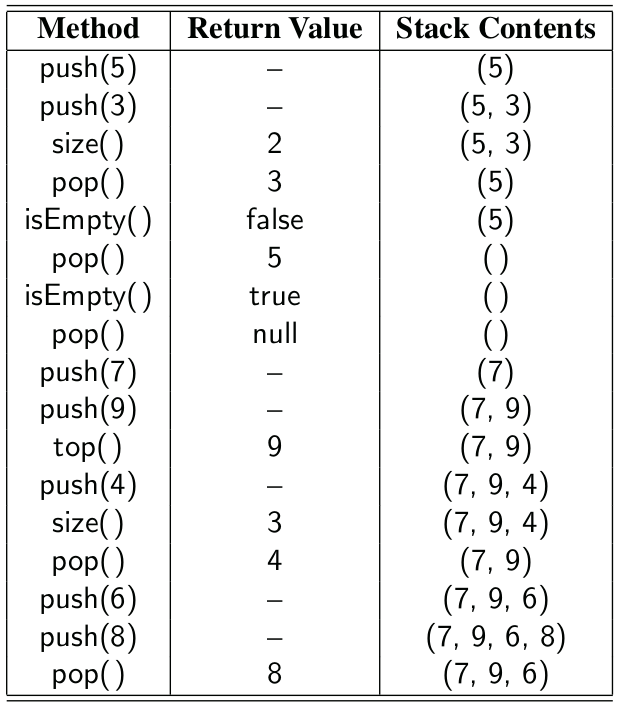
\includegraphics[width=0.43\linewidth]{img/example-6-3}
\end{figure}

\clearpage

Interface \texttt{Stack}:
\begin{minted}{java}
public interface Stack<E> {
	int size();
	boolean isEmpty();
	void push(E e);
	E top();
	E pop();	
}
\end{minted}

\medskip

Implementação baseada em vetor:
\begin{minted}{java}
public class ArrayStack<E> implements Stack<E> {
	public static final int CAPACITY = 1000;
	private E[] data;
	private int t = -1;
	
	public ArrayStack() { this(CAPACITY); }
	
	public ArrayStack(int capacity) {
		data = (E[]) new Object[capacity];
	}
	
	public int size() { return (t + 1); }
	
	public boolean isEmpty() { return (t == -1); }
	
	public void push(E e) {
		if (size() == data.length)
			throw new IllegalStateException("Stack is full");
		data[++t] = e;
	}
	
	public E top() {
		if (isEmpty()) return null;
		return data[t];
	}
	
	public E pop() {
		if (isEmpty()) return null;
		E answer = data[t];
		data[t] = null;
		t--;
		return answer;
	}
}
\end{minted}

\medskip

\begin{itemize}
	\color{redtext}
	\item Comentários:
	\begin{itemize}
		\item Simples.
		\item Eficiente.
		\item Tamanho estático/fixo.
		\begin{itemize}
			\item Desperdício de memória ou impossibilidade de inserção.
		\end{itemize}
	\end{itemize}
\end{itemize}

\medskip

\begin{itemize}
	\item Análise de eficiência:
	\begin{itemize}
		\item \texttt{size}: $O(1)$.
		\item \texttt{isEmpty}: $O(1)$.
		\item \texttt{top}: $O(1)$.
		\item \texttt{push}: $O(1)$.
		\item \texttt{pop}: $O(1)$.
	\end{itemize}
\end{itemize}

\medskip

\underline{Exercícios:}
\begin{enumerate}
	\item Considere um sistema onde o usuário interage através de uma shell, fornecendo os comandos desejados na forma de texto. Implemente uma pilha baseada em vetor para armazenar os comandos informados pelo usuário. Ao digitar o comando '\texttt{sair}', o sistema deve desempilhar os comandos e mostrar ao usuário como log do sistema.
\end{enumerate}

\clearpage

Implementação baseada em listas simplesmente encadeadas:
\begin{minted}{java}
public class LinkedStack<E> implements Stack<E> {
	private SinglyLinkedList<E> list = new SinglyLinkedList<>();
	public LinkedStack() { }
	public int size() { return list.size(); }
	public boolean isEmpty() { return list.isEmpty(); }
	public void push(E element) { list.addFirst(element); }
	public E top() { return list.first(); }
	public E pop() { return list.removeFirst(); }
}
\end{minted}

\medskip

\begin{itemize}
	\color{redtext}
	\item Comentários:
	\begin{itemize}
		\item Operações continuam com complexidade constante $O(1)$.
	\end{itemize}
\end{itemize}

\medskip

\underline{Exercícios:}
\begin{enumerate}
	\item Substitua a pilha utilizada no exercício anterior por uma pilha baseada em uma lista simplesmente encadeada.
	
	\item Utilize pilhas para inverter a ordem dos elementos de um vetor de elementos (de qualquer tipo).
\end{enumerate}

\medskip

\newtitle{Filas}

Ideia geral:
\begin{itemize}
	\item Estratégia \textbf{FIFO}: \textit{first-in-first-out}.
	\item Primeiro elemento a ser inserido é o primeiro a ser removido.
	\item {\color{redtext}Elemento entra no \textit{final} da fila e sai o elemento da \textit{frente} da fila.}
	\item Operações:
	\begin{itemize}
		\item \texttt{enqueue}: insere elemento no final da fila.
		\item \texttt{dequeue}: remove elemento do início da fila.
	\end{itemize}
	\item Aplicações:
	\begin{itemize}
		\item Impressora de rede.
		\item Servidor Web respondendo requisições.
	\end{itemize}
\end{itemize}

\begin{figure}[H]
	\centering
	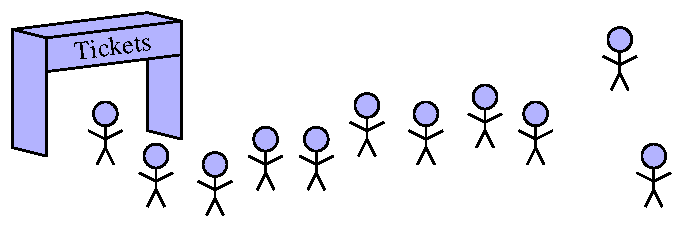
\includegraphics[width=0.5\linewidth]{img/figure-6-4a}
\end{figure}
\vspace{-10pt}
\begin{figure}[H]
	\centering
	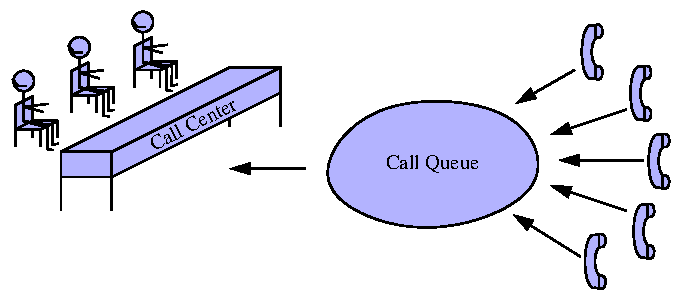
\includegraphics[width=0.5\linewidth]{img/figure-6-4b}
\end{figure}

\begin{itemize}
	\item Exemplo de funcionamento:
	\begin{itemize}
		\item Operações de atualização: \texttt{enqueue}, \texttt{dequeue}.
		\item Operações auxiliares: \texttt{size}, \texttt{first}, \texttt{isEmpty}.
	\end{itemize}
\end{itemize}

\begin{figure}[H]
	\centering
	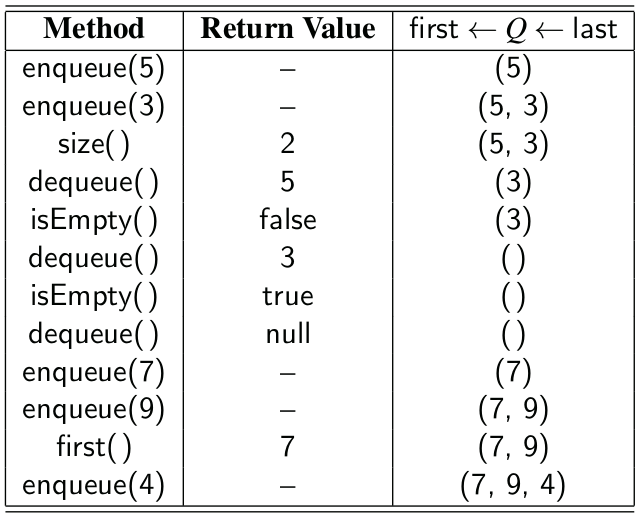
\includegraphics[width=0.45\linewidth]{img/example-6-4}
\end{figure}

\clearpage

Interface \texttt{Queue}:
\begin{minted}{java}
public interface Queue<E> {
	int size();
	boolean isEmpty();
	void enqueue(E e);
	E first();
	E dequeue();	
}
\end{minted}

\medskip

Detalhes de implementação:
\begin{itemize}
	\item Inserção simples no `final' do vetor.
	\item Remoção deve acontecer no início.
	\begin{enumerate}
		\item Remover posição 0 e fazer shift. \inblock{$\gets$ custoso: $O(n)$}
		\item Utilizar uma variável como referência para a frente da fila. \inblock{$\gets O(1)$}
	\end{enumerate}
\end{itemize}

\medskip

Ideia geral:
\begin{figure}[H]
	\centering
	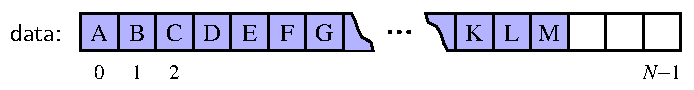
\includegraphics[width=0.7\linewidth]{img/figure-6-5}
\end{figure}

Remoção utilizando variável $f$:
\begin{figure}[H]
	\centering
	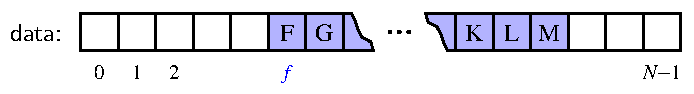
\includegraphics[width=0.7\linewidth]{img/figure-6-6}
\end{figure}

\medskip

Novo desafio: deve-se controlar espaços vagos no início do vetor.

\begin{figure}[H]
	\centering
	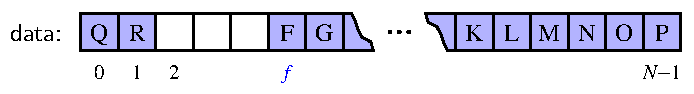
\includegraphics[width=0.7\linewidth]{img/figure-6-7}
\end{figure}

\underline{Solução:} implementar uma estratégia circular, cujo incremento na última posição leva à primeira.

\medskip

Implementação baseada em vetores:
\begin{minted}{java}
public class ArrayQueue<E> implements Queue<E> {
	public static final int CAPACITY = 1000;
	private E[] data;
	private int f = 0;
	private int sz = 0;
	
	public ArrayQueue() {this(CAPACITY);}
	
	public ArrayQueue(int capacity) {
		data = (E[]) new Object[capacity];
	}
	
	public int size() { return sz; }
	public boolean isEmpty() { return (sz == 0); }
	
	public void enqueue(E e) {
		if (sz == data.length) 
			throw new IllegalStateException("Queue is full");
		
		int avail = f + sz;
		if(avail >= data.length) avail -= data.length;
		
		data[avail] = e;
		sz++;
	}
	
	public E first() {
		if (isEmpty()) return null;
		return data[f];
	}
	
	public E dequeue() {
		if (isEmpty()) return null;
		E answer = data[f];
		data[f] = null;
		
		f = (f + 1);
		if(f >= data.length) f = 0;
		
		sz--;
		return answer;
	}
}
\end{minted}

\medskip

\begin{itemize}
	\item Análise de eficiência:
	\begin{itemize}
		\item \texttt{size}: $O(1)$.
		\item \texttt{isEmpty}: $O(1)$.
		\item \texttt{first}: $O(1)$.
		\item \texttt{enqueue}: $O(1)$.
		\item \texttt{dequeue}: $O(1)$.
	\end{itemize}
\end{itemize}

\medskip

Implementação baseada em listas simplesmente encadeadas:
\begin{minted}{java}
public class LinkedQueue<E> implements Queue<E> {
	private SinglyLinkedList<E> list = new SinglyLinkedList<>();
	public LinkedQueue() { }
	public int size() { return list.size(); }
	public boolean isEmpty() { return list.isEmpty(); }
	public void enqueue(E element) { list.addLast(element); }
	public E first() { return list.first(); }
	public E dequeue() { return list.removeFirst(); }
}
\end{minted}

\medskip

\begin{itemize}
	\color{redtext}
	\item Comentários:
	\begin{itemize}
		\item Operações continuam com complexidade constante $O(1)$.
	\end{itemize}
\end{itemize}

\underline{Exercícios:}
\begin{enumerate}
	\item Implemente uma fila baseada em vetor para armazenar os pacientes de um plantão de atendimento. Sempre que o paciente chega, um atendente faz seu cadastro, informando nome, idade e código do plano de saúde. O médico de plantão, que possui acesso ao mesmo sistema, efetua a chamada do próximo paciente.
	
	\item Modifique a implementação do exercício anterior, utilizando uma fila baseada em uma lista simplesmente encadeada.
\end{enumerate}

\medskip

\newtitle{Deques}

Ideia geral:
\begin{itemize}
	\item Deque é o termo usado para \textit{double-ended queue}.
	\item Fila com inserção e remoção dos dois lados (início e fim).
	\item Operações:
	\begin{itemize}
		\item \texttt{addFirst}/\texttt{addLast}: insere elemento no início/final.
		\item \texttt{removeFirst}/\texttt{removeLast}: remove o primeiro/último elemento.
	\end{itemize}
\end{itemize}

\begin{itemize}
	\item Exemplo de funcionamento:
\end{itemize}

\begin{figure}[H]
	\centering
	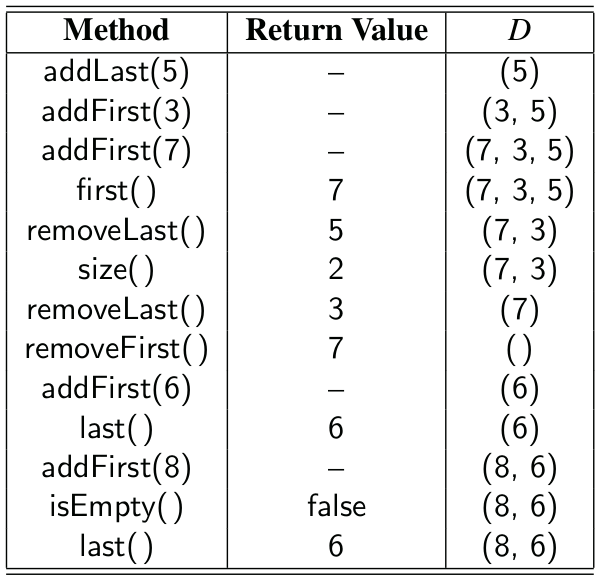
\includegraphics[width=0.38\linewidth]{img/example-6-5}
\end{figure}

Interface \texttt{Deque}:
\begin{minted}{java}
public interface Deque<E> {
	int size();
	boolean isEmpty();
	E first();
	E last();
	void addFirst(E e);
	void addLast(E e);
	E removeFirst();
	E removeLast();
}
\end{minted}

\medskip

Implementação baseada em vetores:
\begin{minted}{java}
public class ArrayDeque<E> implements Deque<E> {
	public static final int CAPACITY = 1000;
	private E[] data;
	private int f = 0;
	private int sz = 0;
	
	public ArrayDeque() {this(CAPACITY);}
	
	public ArrayDeque(int capacity) {
		data = (E[]) new Object[capacity];
	}
	
	public int size() { return sz; }
	public boolean isEmpty() { return (sz == 0); }
	
	public E first() {
		if (isEmpty()) return null;
		return data[f];
	}
	
	public E last() {
		if (isEmpty()) return null;
		int index = f + sz - 1;
		if(index >= data.length) index -= data.length;
		return data[index];
	}
	
	public void addFirst(E e) {
		if (sz == data.length) 
			throw new IllegalStateException("Queue is full");
		
		int avail = f - 1;
		if(avail < 0) avail = data.length - 1;
		
		data[avail] = e;
		f = avail;
		sz++;
	}
	
	public void addLast(E e) {
		if (sz == data.length) 
			throw new IllegalStateException("Queue is full");
		
		int avail = f + sz;
		if(avail >= data.length) avail -= data.length;
		
		data[avail] = e;
		sz++;
	}
	
	public E removeFirst() {
		if (isEmpty()) return null;
		E answer = data[f];
		data[f] = null;
		
		f = f + 1;
		if(f >= data.length) f = 0;
		
		sz--;
		return answer;
	}
	
	public E removeLast() {
		if (isEmpty()) return null;
		int index = f + sz - 1;
		if(index >= data.length) index -= data.length;
		
		E answer = data[index];
		data[index] = null;
		
		sz--;
		return answer;
	}
}
\end{minted}

\medskip

\begin{itemize}
	\color{redtext}
	\item Comentários:
	\begin{itemize}
		\item Todas as operações são realizadas em tempo constante $O(1)$.
		\item Operador módulo controla a lista circular.
	\end{itemize}
\end{itemize}

\medskip


Implementação baseada em listas duplamente encadeadas:
\begin{minted}{java}
public class LinkedDeque<E> implements Deque<E> {
	private DoublyLinkedList<E> list = new DoublyLinkedList<>();
	public int size() { return list.size(); }
	public boolean isEmpty() { return list.isEmpty(); }
	public E first() { return list.first(); }
	public E last() { return list.last(); }
	public void addFirst(E e) { list.addFirst(e); }
	public void addLast(E e) { list.addLast(e); }
	public E removeFirst() { return list.removeFirst(); }
	public E removeLast() { return list.removeLast(); }
}
\end{minted}

\medskip

\begin{itemize}
	\color{redtext}
	\item Comentários:
	\begin{itemize}
		\item Operações continuam com complexidade constante $O(1)$.
	\end{itemize}
\end{itemize}

\clearpage

\underline{Exercícios:}
\begin{enumerate}
	\item Deseja-se armazenar um conjunto de livros para doação. Cada livro doado é inserido no catálogo, e cada pessoa interessada recebe um livro. Implemente uma estrutura de deque, onde cada livro recebido é armazenado em um lado aleatório da lista (início ou fim), e cada pessoa interessada escolhe um dos dois livros dos terminais da lista, o qual é retirado da mesma. Utilize uma implementação de deque baseada em vetores.
	
	\item Modifique o exercício anterior e substitua a implementação do deque por uma baseada em listas duplamente encadeadas.
\end{enumerate}

\medskip

\newtitle{Atividades}

\begin{enumerate}
	\item Resolva os seguintes exercícios de~\cite{GoodrichEtAl2014}:

	\begin{itemize}
		\item[R-6.1:] Suponha que inicialmente uma pilha vazia \texttt{S} tenha realizado um total de $25$ operações \texttt{push}, $12$ operações \texttt{top} e $10$ operações \texttt{pop}, $3$ das quais retornaram \texttt{null}, indicando uma pilha vazia. Qual é o tamanho atual de \texttt{S}?
		
		\item[R-6.2:] Sendo a pilha do exercício anterior uma instância da classe \texttt{ArrayStack}, qual seria o valor final da variável \texttt{t}? 
		
		\item[R-6.3:] Quais valores são retornados durante as seguintes operações, se executado inicialmente em uma pilha vazia? \texttt{push(5)}, \texttt{push(3)}, \texttt{pop()}, \texttt{push(2)}, \texttt{push(8)}, \texttt{pop()}, \texttt{pop()}, \texttt{push(9)}, \texttt{push(1)}, \texttt{pop()}, \texttt{push(7)}, \texttt{push(6)}, \texttt{pop()}, \texttt{pop()}, \texttt{push(4)}, \texttt{pop()}, \texttt{pop()}.
		
		\item[R-6.4:] Implemente um método com a assinatura \texttt{transfer(S, T)} que transfere todos os elementos da pilha \texttt{S} para a pilha \texttt{T}, de modo que o elemento que iniciou no topo de \texttt{S} é o primeiro elemento a ser inserido em \textsl{T}, e o último elemento de \textsl{S} termina no topo de \textsl{T}.
		
		\item[R-6.5:] Apresente um método recursivo que remove todos os elementos de uma pilha.
		
		\item[R-6.7:] Suponha que uma fila vazia \texttt{Q} realizou um total de $32$ operações de \texttt{enqueue}, $10$ operações \textit{first} e $15$ operações \texttt{dequeue}, $5$ das quais retornaram \texttt{null}, indicando uma fila vazia. Qual é o tamanho atual de \texttt{Q}?
		
		\item[R-6.8:] Sendo a fila do exercício anterior uma instância da classe \texttt{ArrayQueue} com uma capacidade de $30$ elementos nunca excedida, qual seria o valor final da variável \texttt{f}?
		
		\item[R-6.9:] Quais são os valores retornados após as seguintes operações, se executadas em uma fila inicialmente vazia? \texttt{enqueue(5)}, \texttt{enqueue(3)}, \texttt{dequeue()}, \texttt{enqueue(2)}, \texttt{enqueue(8)}, \texttt{dequeue()}, \texttt{dequeue()}, \texttt{enqueue(9)}, \texttt{enqueue(1)}, \texttt{dequeue()}, \texttt{enqueue(7)}, \texttt{enqueue(6)}, \texttt{dequeue()}, \texttt{dequeue()}, \texttt{enqueue(4)}, \texttt{dequeue()}, \texttt{dequeue()}.
		
		\item[R-6.10:] Faça um adaptador simples (classe) que implemente uma pilha usando uma instância de deque para armazenamento.
		
		\item[R-6.11:] Faça um adaptador simples (classe) que implemente uma fila usando uma instância de deque para armazenamento.
		
		\item[R-6.12:] Quais são os valores retornados após as seguintes operações, se executadas em um deque inicialmente vazio? \texttt{addFirst(3)}, \texttt{addLast(8)}, \texttt{addLast(9)}, \texttt{addFirst(1)}, \texttt{last()}, \texttt{isEmpty()}, \texttt{addFirst(2)}, \texttt{removeLast()}, \texttt{addLast(7)}, \texttt{first()}, \texttt{last()}, \texttt{addLast(4)}, \texttt{size()}, \texttt{removeFirst()}, \texttt{removeFirst()}.
		
		\item[R-6.13:] Suponha que você tenha um deque \texttt{D} contendo os números (1, 2, 3, 4, 5, 6, 7, 8), nessa ordem. Supondo que além disso você tenha uma fila \texttt{Q} incialmente vazia. Apresente um pseudocódigo que utilize somente \texttt{D} e \texttt{Q} (mais nenhuma variável) e resulte em \texttt{D} armazenando os elementos na ordem (1, 2, 3, 5, 4, 6, 7, 8).
		
		\item[R-6.14:] Repita o exercício anterior usando o deque \texttt{D} e uma pilha \texttt{S}, inicialmente vazia.
	\end{itemize}
\end{enumerate}

\clearpage
\medskip

\newtitle{Referências}
\begingroup
	\footnotesize
	\renewcommand{\chapter}[2]{}%
	\bibliographystyle{apalike}
	\bibliography{../referencias}
\endgroup

\end{document}